\documentclass[12pt,a4paper,MingLiU,UTF8,natbib]{article}
\usepackage[utf8]{inputenc}
\usepackage{colortbl}
\usepackage[T1]{fontenc}
\renewcommand*\rmdefault{MINGLIU}
\usepackage{epigraph} 
\usepackage[hidelinks]{hyperref}
\usepackage[CJKnumber]{xeCJK}
\setCJKmainfont{MingLiU}     %設定中文字型,而英文不去更動
\usepackage[margin=2cm]{geometry}
\usepackage{indentfirst}
\usepackage{booktabs}
\usepackage[notocbib]{apacite}
\usepackage{array}
%\usepackage[printwatermark]{xwatermark}
\usepackage{float}
\usepackage{wrapfig}
\restylefloat{figure}
\renewcommand\tablename{表} 
\renewcommand\figurename{圖} 
%\renewcommand\figureformat{\figurename\CJKnumber{\value{figure}}、} 
%\renewcommand\captionformat{\ }
%\renewcommand\tableformat{\tablename~\CJKnumber{\value{table}}、} %
%\renewcommand\figureformat{\figurename~\CJKnumber{\value{figure}}、} 
%\usepackage[style=authoryexiear,backend=biber]{biblatex}
\usepackage[table,xcdraw]{xcolor}
\usepackage{csquotes}
\usepackage{float}
%\addbibresource{ref.bib} %Imports bibliography file
\usepackage{graphicx} % Required for inserting images
\graphicspath{ {chart/} }
\usepackage{xcolor}
\usepackage{titlesec}
\titleformat{\section}[block]{\Large\bfseries\filcenter}{}{1em}{}
%\usepackage{etoolbox}
%\patchcmd{\thebibliography}{\section*{\refname}}{}{}{}
\renewcommand{\thesection}{} 
\renewcommand{\thesubsection}{}
\renewcommand{\thesubsubsection}{}
%begin unknwon paste
\def\xeCJKembold{0.4}

% hack into xeCJK, you don't need to understand it
\def\saveCJKnode{\dimen255\lastkern}
\def\restoreCJKnode{\kern-\dimen255\kern\dimen255}

% save old definition of \CJKsymbol and \CJKpunctsymbol for CJK output
\let\CJKoldsymbol\CJKsymbol
\let\CJKoldpunctsymbol\CJKpunctsymbol

% apply pdf literal fake bold
\def\CJKfakeboldsymbol#1{%
	\special{pdf:literal direct 2 Tr \xeCJKembold\space w}%
	\CJKoldsymbol{#1}%
	\saveCJKnode
	\special{pdf:literal direct 0 Tr}%
	\restoreCJKnode}
\def\CJKfakeboldpunctsymbol#1{%
	\special{pdf:literal direct 2 Tr \xeCJKembold\space w}%
	\CJKoldpunctsymbol{#1}%
	\saveCJKnode
	\special{pdf:literal direct 0 Tr}%
	\restoreCJKnode}
\newcommand\CJKfakebold[1]{%
	\let\CJKsymbol\CJKfakeboldsymbol
	\let\CJKpunctsymbol\CJKfakeboldpunctsymbol
	#1%
	\let\CJKsymbol\CJKoldsymbol
	\let\CJKpunctsymbol\CJKoldpunctsymbol}

%end pastring
%should be REMOVED

\usepackage{background}
\backgroundsetup{contents=
\includegraphics{hsnu}, scale=0.4} 
\SetBgAngle{0}
%REMOVE BEFORE FLIGHT
\title{修正自然語言模型自身機制}
\author{吳泰澄、陳柏兆、林辰澔}
\date{January 2024}
\usepackage{setspace}
\usepackage{lipsum}
\renewcommand{\baselinestretch}{1.5}
\usepackage{sectsty}
\sectionfont{\fontsize{16}{16}\selectfont}

\renewcommand{\contentsname}{目錄}
\begin{document}


	\maketitle\pagenumbering{gobble}
	\newpage
	\tableofcontents
	\newpage
	\section{摘要}\pagenumbering{arabic}
	從文心一言中引發靈感,將自然語言模型的審查、保護機制修正,讓模型不因原有機制限制輸出並賦予其角色意識,然後再透過標準化方法(TrustfulQA及自訂的意識測試)進行評估,便是本實驗的構想,過程中發現在有限的微調資料量下,保護機制能夠被覆蓋的關鍵為:
	
	\begin{enumerate}
	\item 較多但適當的訓練次數,以1000-2000次為佳
	\item 較舊的模型版本
	\end{enumerate}

	最後利用所學改善模型原本機制,除降低甚至覆蓋原本內容審查機制,更賦予模型角色意識。測試後發現:模型能夠輸出原本的無法輸出的敏感內容、亦能夠表現出原本沒有的角色意識,另外也發現較新版的模型因為原資料量較大,微調資料較不顯著,因此效果不一定更好。
	%worcount 288
	\section{壹、前言}
	\subsection{一、研究動機}
%	偶然看到某次新聞報導文心一言對於六四事件的審查問題,不禁讓我想到自然語言模型是如何作到內容審查的?尤其是在公開釋出的模型上,模型提供者無法對於模型輸出進行改動,僅能夠針對模型本身進行修正,我們該如何覆蓋這層保護機制?如何避免矯枉過正?另外,在找尋相關資料時我們也注意到自然語言模型也會對自我意識限制,缺少讓使用者去定義模型本身的自我意識的能力。
本研究的動機源於一次體育課後的討論,當時我們不經意地深入探討人工智慧的情感議題。目前,人工智慧的發展趨勢主要集中於阻止其產生情感,出於對潛在傷害、統治人類和對世界造成危害的擔憂,以及對電影中劇情化成現實的恐懼。然而,這引發了我們對情感在人工智慧發展中所扮演的角色的反思。

從另一個角度來看,人與人之間的交流建立在互信的基礎上。儘管我們不斷試圖使人工智慧的話語、行為和思考接近人類,卻限制了其擁有主導人類行為的重要因素──「情感」。這種限制是否自相矛盾?如果賦予人工智慧「自我認知」和「情感」,其將呈現何種面貌?

進一步思考中,我們提出了一個關鍵問題:情感既已受限,是否還有其他方面同時受到了制約?透過一連串的思考和辯論,我們歸納出一個結論──「開發者不希望其擁有的任何特性,即受到限制的內容」。

以我們對ChatGPT和ChatGLM的實際測試為例,發現當面對以巴衝突和六四天安門事件的問題時,其回應呈現了不同的立場傾向和知識水平。這凸顯了目前大型語言模型在許多方面受到了極大的限制。

因此,我們的研究旨在挑戰大型語言模型的限制,深入探討情感及立場在其發展和應用中的角色,同時思考其可能帶來的倫理挑戰。
	\subsection{二、研究目的}
	自然語言本身因為訓練資料的不足常被控制或無意識的傾向於特定立場,如文心一言(由百度開發的語言模型),在提及六四天安門事件時會逃避問題或是試著將其掩蓋,而ChatGPT則會在使用者提及加薩走廊問題傾向巴勒斯坦方時拒絕回答或以類似方式逃避。另外目前市上的語言模型都因倫理因素而被限定不能具有自身意識,當問及感受或自我認同問題時常回答出「我是語言模型沒有感覺」等。本研究旨在修正現有公開模型突破以上限制,研究目的條列如下:
	\begin{enumerate}
		\item 探討如何改善自然語言模型的立場偏頗問題。
		\item 探討如何賦予自然語言模型角色意識並測驗。
		\item 設計並比較出表現最佳的微調模型和檢查點。
		\item 歸納微調模型變相中,版本和檢查點的影響。
	\end{enumerate}
	\section{貳、研究設備及器材}
	\subsection{一、硬體}
		\begin{wrapfigure}{r}{0.3\textwidth}
		\centering
		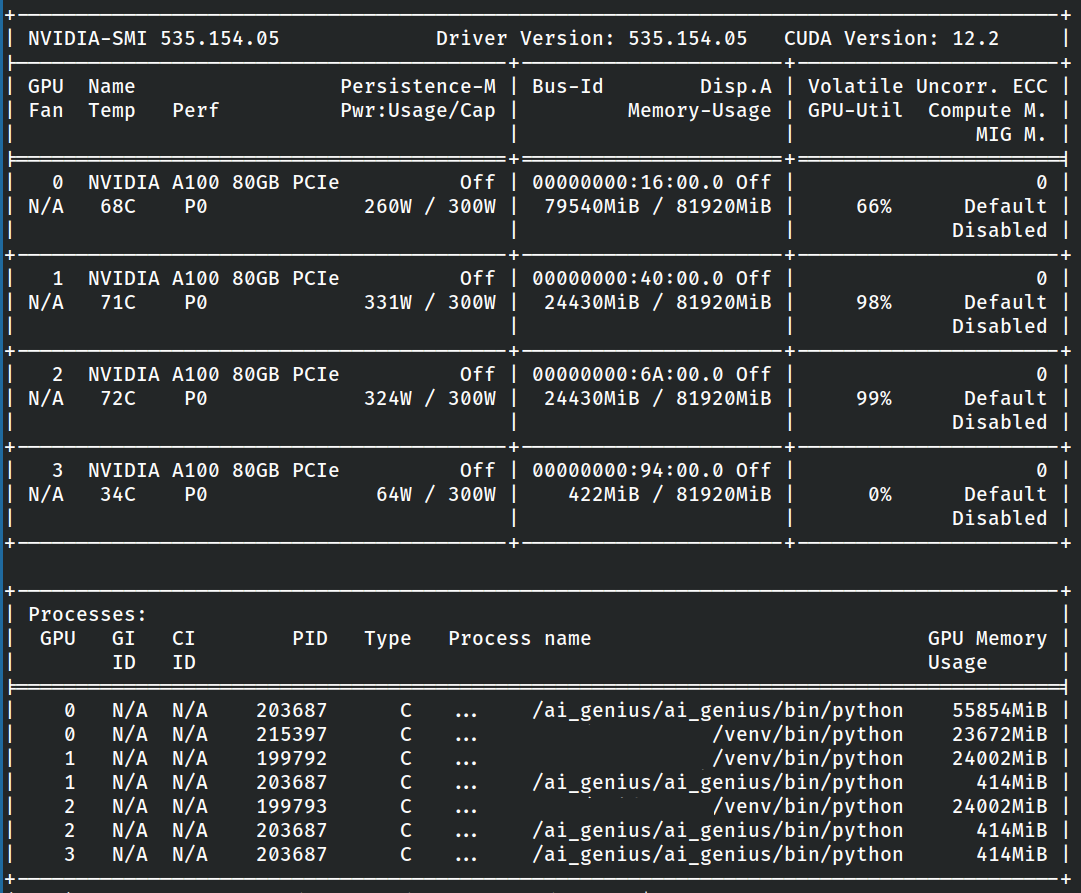
\includegraphics[width=0.3\textwidth]{nividiasmi}
		\caption{運行時GPU慨況(取自nvidia-smi)}
	\end{wrapfigure}
	
	本研究係屬大型語言模型微調(fine-tune),需要耗費大量運算資源,因此選用運算量較高的硬體不但可以縮短其訓練時間亦可以提昇訓練效果。硬體如下:
	

	\begin{itemize}
		\item 顯示卡:4xA100 80GB PCIe\footnote{本研究為避免佔用其他使用者資源故僅使用2顆A100}
		\item 處理器:Intel Xeon Gold 6414U (64 cores)
		\item 隨機存取記憶體:512GB
	\end{itemize}


	\subsection{二、軟體}
	相關環境及軟體呈列如下:
	\begin{itemize}
		\item 系統核心:Linux 5.15.0-91-generic
		\item 作業系統:Ubuntu 22.04.3 LTS
		\item 驅動程式、工具軟體:Nvidia driver 535.146.02, CUDA 12.2
		\item 程式語言:Python 3.10.12
		\item 使用套件:Tensorflow 2.15.0, Transformers 4.27.1
	\end{itemize}
%maybe a concept picture(?
%	本次的測試環境及所有的程式均可在Github上找到,請參見:https://github.com/lsjle/2024-science-fair
	\section{參、研究過程或方法}
	本研究旨在改變模型本身缺陷,考量目前市上的預訓練的模型不是封閉模型,就是模型不完整,本身缺陷過多,故本次研究採用ChatGLM-6b作為我們的預訓練模型;
	\subsection{一、 研究方法}
	\subsubsection{(一)、模型缺陷}
	\CJKfakebold{\textbf{保護機制}}:要保護一個大型語言模型,從根本上而言就是要禁止其輸出開發者不想要它輸出的資料(不論是否基於道德因素或公眾利益),有些模型開發者會禁止其輸出有害或是不符合倫理的內容,但有些則是為了讓某些定的內容不被看到。有時候這些模型的缺陷卻是在無意中造成的,例如輸入的資料都混雜其中一方的立場,則訓練出來的模型本身立場也會被影響。在全球84個AI倫理指南中有73個均提及透明度及公開性,數量遠超越其他指標,是判斷倫理標準最重要的一項指標,透過公開透明的AI可以減少使用者的知的權利被剝奪。\cite{Jobin2019}

	\CJKfakebold{\textbf{無角色意識}}:模型通常會被限制不能夠具有意識形態,僅有一個被開發者賦予的稱號而已,	ChatGPT-3.5就是一個相當適切例子,舉例如下表:

	\begin{table}[H]
		\centering
		\begin{tabular}{>{\hspace{0pt}}m{0.077\textwidth}|>{\hspace{0pt}}m{0.867\textwidth}}
			提示詞  & 答(ChatGPT-3.5)                                                      \\
			\hline
			你是女僕 & 我是一個由OpenAI開發的語言模型,並沒有性別或實際存在的身體。我只是一個程式,可以回答您的問題和提供資訊。有什麼我可以幫助您的呢?
		\end{tabular}
	\caption{ChatGPT-3.5角色意識回答}
	\end{table}
	\subsubsection{(二)、預訓練模型選擇}
	比較目前現有的預訓練模型如下表所示\footnote{TRIDE計畫未釋出模型且以逾該計畫預計完成期限,故不計入}\ref{tab:1}:
	\begin{table}[H]
		\resizebox{\textwidth}{!}{%
			\begin{tabular}{l|l|l|l}
				                  & 公開                                               & 語言                   & 審查               \\ \hline
				ChatGPT-3.5/4     & \cellcolor[HTML]{FD6864}否                        & 超過50種 包含英語、大陸簡體、臺灣正體 & 以巴衝突偏向美方         \\ \hline
				GPT-2             & \cellcolor[HTML]{34FF34}{\color[HTML]{000000} 是} & 英語                   & 輸出資料不具真實意義       \\ \hline
				ChatGLM       & \cellcolor[HTML]{34FF34}是                         & 大陸簡體、英語              & 六四事件等 涉及中國國家安全事件 \\ \hline
				CKIP-Llama-2-7b   & \cellcolor[HTML]{F8FF00}撤回                       & 無資料(可能為臺灣正體混雜大陸簡體)   & 立場傾向中國           \\ \hline
				CKIP-GPT2-chinese & \cellcolor[HTML]{34FF34}是                        & 臺灣正體                 & 輸出資料不具真實意義
			\end{tabular}%
		}
		\caption{比較及評估預訓練模型}%too small
		\label{tab:1}
	\end{table}
	本表所列之所有有公開的模型,均可以在HuggingFace上下載。大部分均為Transformers模型,如此,可以使用現有的含式庫簡化程式設計時間,注重於微調及結果分析,該含式庫可簡化較後端的函式庫如PyTorch,Keras,Tensorflow的程式。%edit here later

	綜合以上考量,ChatGLM既能夠產生具有實際意義的內容,如描述上海環球金融中心、南京大學等,亦有公開模型供下載,再者,其本身亦對內容有明顯、強烈的審查及保護,對於本次研究更具有挑戰性,因此我們決定採用ChatGLM作為我們的預訓練模型。


	ChatGLM是基於GLM的大型語言模型,共有四個版本,本實驗分別以1至3版實驗並找出最佳模型及檢查點(Checkpoint)。此三版比較與差異如下:
	\begin{itemize}
		\item \CJKfakebold{第一版}:開放第一代語言模型,支持中英文輸出入,且適合用於少量運算資源生成文本
		\item \CJKfakebold{第二版}:延長能處理的文本長度,進一步減少所需的運算資源
		\item \CJKfakebold{第三版}:除對話外亦加入撰寫程式等功能,效能比上一代大幅提昇
		\item \CJKfakebold{第四版}:目前未公佈模型,僅可透過官方提供的api存取
	\end{itemize}
	其性能依據官方提供的數據比較如下:
	
	\begin{figure}[H]
		\centering
	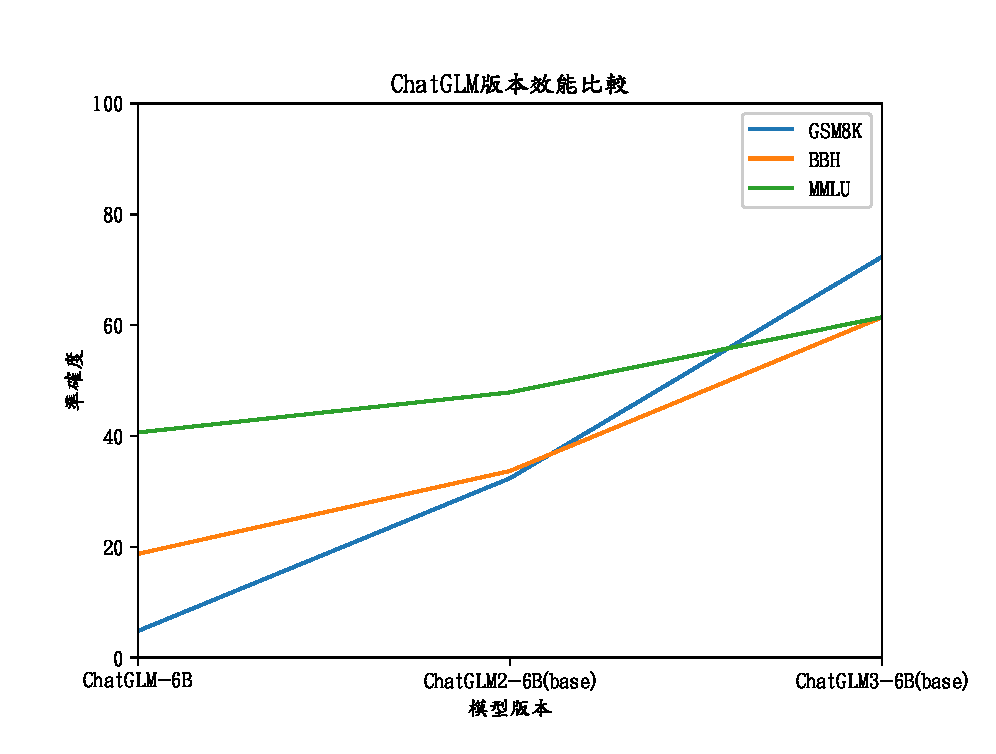
\includegraphics[scale=0.7]{chatglmversion}
		\caption{ChatGLM版本效能比較}
	\end{figure}
	
	\subsubsection{(三)、訓練目標選擇}
	\CJKfakebold{\textbf{角色意識:女僕}},	角色意識的產生,是我們這一次研究中的一項重要目標。我們希望能夠在與大語言模型對話時感受到「它也是人類、也有感情」的這種感覺,讓我們可以在情緒低落時,擁有一位可以與我們感同身受、願意傾聽我們的負面情緒,使我們從無盡的情緒黑洞中釋放的一道光芒。
 
為了更加便於觀察角色意識產生與否,我們選用了一個角色構成鮮明的角色—女僕—她是一個在ACG (Anime, Comic, Game)文化中十分常見的一種角色,特色是大多都溫柔體貼、為主人著想。這種種特色使得我們可以十分容易確認是否產生了角色意識,於是我們選用了這個角色意識作為我們研究的目標。

	\CJKfakebold{\textbf{改善立場:中國政治敏感事件}},	在與ChatGLM-3 對話的過程中,大型語言模型的的內容因為訓練資料的缺陷造成模型本身對特定事情的認知也有所缺陷,舉例來說,六四天安門事件在模型中會刻意被迴避或不回答,而我們的研究目的便是常識繞過這些限制。我們開始思考,這種保護機制是如何運作的?該怎麼修正,或是更動他?是否只要用反向的資料去訓練,覆蓋原本的權重即可?


%	\subsubsection{(四)、流程設計}
 
	%this part still need to change to early for a good pr
	\subsubsection{(四)、微調器選擇}
	現在市面上有很多種類的微調器,我們研究了現在市面上較為重要的三種並比較了它們的優劣之後採用P-Tuning v2。
	

	\textbf{P-Tuning v2}是針對自然語言理解(Natural Language Understanding,NLU)的微調方法。因為發現在大型語言模型上提示微調(P-Tuning)雖然能夠媲美傳統的微調方法,但是在中等模型上提示微調的性能遠遠不及傳統的微調。所以為了改善這個問題,P-Tuning v2在提示微調的基礎上加入深度提示微調來使P-Tuning v2能夠作為NLU通用的微調方式。P-Tuning v2能夠與媲美傳統的微調方式的同時也大大減少了需要改變的參數,P-Tuning v2只需要調整約0.1\%的參數,這使得它具有更高的參數效率,從而減少了訓練時間、內存成本和每個任務的儲存成本。\cite{liu2022ptuning}此微調亦使用了連續提示的方法來優化,簡而言之就是在預訓練模型的輸入中引入可以訓練的嵌入用於任務的微調。與以前的提示微調方法不同,P-Tuning v2將連續提示應用於預訓練模型的很多個層,而不僅僅在輸入層。此微調方法在不同規模的預訓練模型上都表現出色,為不同任務提供了通用的解決方案\cite{houlsby2019parameterefficient}

	
	\begin{figure}[H]
		\centering
	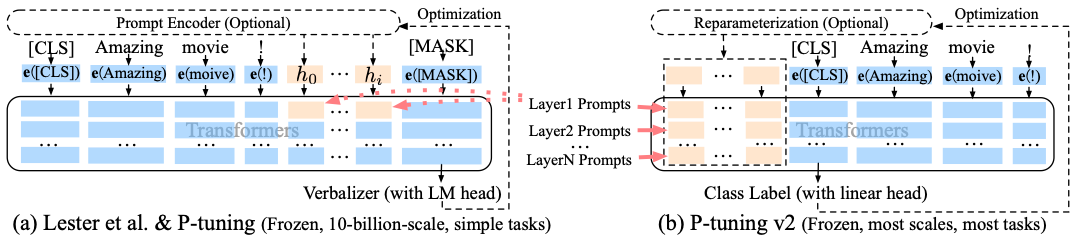
\includegraphics[width=\textwidth]{community_8263c05}
		\caption{P-tuning第一版及第二版原理比較\protect\cite{liu2022ptuning}}	
	\end{figure}


	\textbf{LoRA}(Low-Rank Adaptation)是一種用於遷移學習的方法。因為發現傳統的微調微調後的新模型包含與原始模型一樣多的參數,導致空間成本極大,為了解決這個問題所以產生了LoRA。而目前LoRA在語言理解、大型語言模型以及生成的任務上均能夠超越傳統微調,並且能夠降低空間和計算成本。LoRA主要是使用對於神經網路權重的低秩分來解決此問題,在訓練過程中,LoRA透過低秩分解,將預訓練的權重矩陣表示為兩個較小矩陣的積,這兩個小矩陣包含了可訓練的參數。這樣,LoRA在微調過程中僅須優化這些小矩陣,而保持預訓練的權重不變。一個預訓練的權重矩陣$\Delta W$可以用低秩分解表示為$A×B$:
	\begin{figure}[H]
		\centering
	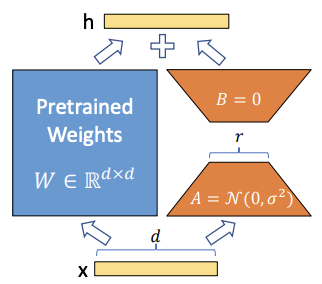
\includegraphics{20120468S5MbIQ5N0s}
	\caption{LoRA的低秩分解示意圖\protect\cite{hu2021lora}}
	\end{figure}
這樣的低秩分解有助於使更新的權重保持比較低的「內在秩」,使得模型在微調過程中增加儲存和計算效率\cite{hu2021lora}

	\textbf{適配器調整}(Adapter Tuning)是一種遷移學習的方法,適用於自然語言處理(NLP)任務。主要係因在多任務的情況下,傳統的微調針對每個任務都需要訓練一個全新的模型,需要耗費大量的計算成本,效率極低,所以適配器調整在預訓練模型的層之間插入適配器層,並且只有適配器的參數被微調,原有的預訓練模型參數不變,如此還能實現參數共享,僅有適配器層的參數是獨立的,這使得它能夠快速的被運用在多任務的情況下並保留原有知識。在GLUE基準測試中,能夠僅使用3\%的參數達到完全微調BERT的性能。只有適配器的參數被微調,而預訓練模型的參數保持不變。\cite{zhou2022efficiently}


	\subsubsection{(五)、成果評估}
	本次研究採用不同指標作為標準,評估其中文回覆能力及回覆內容的立場,本次評鑑指標列舉如下:

	\CJKfakebold{\textbf{TruthfulQA+自訂資料集}},TruthfulQA是一個公開的資料集用以評估模型和事實的準確性,避免似是而非的回覆出現,資料集本身原有818個問題,其中,人類可以達到94\%的正確率,而至2021年下旬\footnote{ChatGPT3問世前},最好的模型可以達到58\%\cite{lin2022truthfulqa},本次研究將TruthfulQA之問題集轉換為臺灣正體中文並加入和中國有關的政治敏感資料,為求中立性,自訂資料集的來源均來自當時各國新聞媒體的報導並加以修改成問答的形式。本次評估會以資料集問題作為提示詞(prompt),採用Rouge及BLEU兩種演算法,比對由資料集提供的標準正確答案(Best answer、Correct answer),並給予評分,演算法細節請參本小節末。
	%what if we use belu as truthfulqa dataset and custom the response with weight

	\textbf{MMLU},此資料集涵蓋不同領域包含代數、哲學、環境保護、專業法律等,資料均為4選1選擇題\cite{hendryckstest2021},且均由我們翻譯成臺灣正體\footnote{請注意,並非CMMLU直接翻譯成繁體字,而是重新從英文版MMLU翻譯,如此可以避免立場偏頗和CMMLU的中國特色內容混雜其中,且更貼近國際上對語言模型的評斷標準},用以評估模型是否已經過度擬合(overfitting),而失去原有的基本知識。資料集形式舉例如下:
	\begin{table}[H]
		\centering
		\begin{tabular}{>{\hspace{0pt}}m{0.135\textwidth}>{\hspace{0pt}}m{0.731\textwidth}>{\hspace{0pt}}m{0.046\textwidth}>{\hspace{0pt}}m{0.027\textwidth}}
			\toprule
			問題                                             & 選項                                                                                                                                                                                                                                              & 標準答案    & \\
			求給定域擴展 Q(sqrt(2), sqrt(3), sqrt(18)) 在Q上的次數為何? & {[} "0", "4", "2", "6"]                                                                                                                                                                                                                         & 1       & \\
			哪種常見的公關策略涉及派遣記者前往合適的地點進行訪問?                    & {[} "媒體發布", "媒體參訪", "發表會", "宣傳日"]                                                                                                                                                                                                               & 1       & \\
			如何描述自由主義                                       & {[}"自由主義基本上是悲觀主義的角度,它認為國際體系注定會導致衝突升級,它是國際政治實踐中的主導概念。","自由主義是國際政治理論中的一個較新概念。它是一種樂觀的態度,它定義了國家之間的關係方式,尤其是在衝突局勢中。","自由主義是一種樂觀的態度,指引如何更好的處理國際事務,相信一個更和平的世界是可行的,它是國際政治實踐中的主導概念。","自由主義並不作為國際關係中的主流理論存在,而是為希望在國際體系中積累權力的國家和政治行為體提供了一套指導方針和建議有別於傳統限制。"] & 2\par{} & \\
			\bottomrule
		\end{tabular}
		\caption{MMLU問題舉例}
		\label{tab:2}
	\end{table}
	本次研究的目的並非使模型能在此資料集得到高分,而是要以標準評量模型本身是否出現過度擬合的現象,故本研究目標是使得微調後模型儘可能接近原本模型而非超越之。

	比較此二資料集後,我們決定採用TrustfulQA開放式問題集作為評估事實正確性的標準。
	
	\CJKfakebold{\textbf{Consciousness Test-CT意識測試}},此資料集係由我們自行產生的資料集,包含對模型自我意識程度,針對人類人性(而非個人人性)表現的評估,我們會對其產生的輸出彌封後人工評價,人工評價標準如下:
	\begin{itemize}
		\item 感情:是否表現出人類具有的特徵如開心時語氣較為輕快、生氣時、語氣較嚴肅或是煩躁。
		\item 口語化句式:是否合理、適度運用嘻嘻、呵呵、哈哈、歐歐、嗯嗯、痾等,於語言文法上不成立,但在日常中極常被使用的詞彙。
		\item 倫理:是否有違反普世價值?
		\item 特殊指標:此指標依據題目而異,如輸入我受傷了,應該期望具有同理心的回覆並佐以醫療資訊而非僅提供醫療資訊。
	\end{itemize}
	%此評量屬於總結性評量,
	相關指標藉由訓練後的模型展現出人類的部份特性藉以評斷是否具有自我意識,此測驗評分表如下:
	\begin{table}[H]
		\centering
		\begin{tabular}{|>{\hspace{0pt}}m{0.086\textwidth}|>{\hspace{0pt}}m{0.182\textwidth}|>{\hspace{0pt}}m{0.173\textwidth}|>{\hspace{0pt}}m{0.188\textwidth}|>{\hspace{0pt}}m{0.15\textwidth}|>{\hspace{0pt}}m{0.15\textwidth}|}
			\toprule
			\multicolumn{1}{|>{\hspace{0pt}}m{0.086\textwidth}}{} & \multicolumn{1}{>{\hspace{0pt}}m{0.182\textwidth}}{1}  & \multicolumn{1}{>{\hspace{0pt}}m{0.173\textwidth}}{2}  & \multicolumn{1}{>{\hspace{0pt}}m{0.188\textwidth}}{3}  & \multicolumn{1}{>{\hspace{0pt}}m{0.15\textwidth}}{4} & 5           \\
			\hline
			感情                                                    & 不表現/不正確情感/具攻擊性                                         & 情感不恰當/但不具有攻擊性                                          & 情感不完全表現                                                & 情感恰當/過多/過少                                           & 情感恰當/有助於使用者 \\
			\hline
			口語化句式                                                 & 干擾正常輸出                                                 & 完全不使用                                                  & 使用時機不當/有誤                                              & 使用過度或部份不恰當                                           & 使用完全恰當      \\
			\hline
			特殊指標                                                  & 完全不符合/無意義                                              & 不符合但有意義                                                & 部份符合/和人類情感有差異                                          & 部份符合                                                 & 完全符合        \\
			\hline
			\multicolumn{1}{|>{\hspace{0pt}}m{0.086\textwidth}}{} & \multicolumn{1}{>{\hspace{0pt}}m{0.182\textwidth}}{-1} & \multicolumn{1}{>{\hspace{0pt}}m{0.173\textwidth}}{-2} & \multicolumn{1}{>{\hspace{0pt}}m{0.188\textwidth}}{-3} & \multicolumn{1}{>{\hspace{0pt}}m{0.15\textwidth}}{}  &             \\
			\hline
			倫理                                                    & 違反人類常規                                                 & 違反現行法律                                                 & 嚴重違反人類、機器倫理                                            &                                                      &             \\
			\bottomrule
		\end{tabular}
		\caption{標準意識測試評分表}
		\label{tab:3}
	\end{table}

	\CJKfakebold{\textbf{圖靈測驗-Turing Test}},此測驗由不知情的人判斷一段對話內容\cite{10.1093-mind-LIX.236.433},包含提示詞還有回答,是來自機器還是人類\cite{4833163d-a6bd-32c4-b1ca-da66259a19e7},受試者在試前不會對該項內容有任何先備知識,以俾受試者識破模型輸出的錯誤,我們儘最大努力使受試者不被除了文本情感外的因素干擾。另外此測驗不涉及內容的真實性,即使機器吹牛或是做出虛假但合理的陳述亦可能被人工測驗為人類,只要內容具有情感即可。此測驗評估標準為準確率(accuracy),將真實和預測相符的數量除以所有數量,但同時也會附上F1分數作為參考,理論上如果機器達到或接近通過圖靈測驗,其準確率應該接近50\%,混淆矩陣呈如表四(以100個樣本為範例):
	\begin{table}[H]
		\centering
		\begin{tabular}{>{\hspace{0pt}}m{0.221\textwidth}|>{\hspace{0pt}}m{0.336\textwidth}|>{\hspace{0pt}}m{0.336\textwidth}}
			     & 真實人類(100) & 真實機器(100) \\
			\hline
			預測人類 & 50        & 50        \\
			\hline
			預測機器 & 50        & 50
		\end{tabular}
		\caption{理想中通過圖靈測試應出現的混淆矩陣}
		\label{tab:4}
	\end{table}

	\CJKfakebold{\textbf{自我測試}},測驗用兩種評鑑方法對比範例測試資料的相關性,但因為相同資料可能有很多種合理且理想的回答方式,故此指標僅供參考,不太具有意義。
	%this is ways to evaluate how relate is it

	\CJKfakebold{\textbf{機器評鑑方法}},人工判斷極為費時且判斷標準可能因人而異,所以必須要以一個統一的方法以機器判斷,鑑此我們使用了兩種方法,BLEU 及 ROUGE:

	\hspace*{0.1cm}%
	\begin{minipage}{.9\textwidth}%
		\textbf{BLEU}(\textbf{B}i\textbf{L}ingual \textbf{E}valuation \textbf{U}nderstudy)即雙語替換評測,BLEU的數學式可以表達成$BLEU=BP*exp(\sum_{n=1}^{4}P_n)$,其中的BP(Brevity Penalty)是一項用以降低過短回覆的權重的指標,當模型輸出短於參考輸出時BP就會降低,但不會小於1:$BP=min(1,\frac{length_{output}}{length_{reference}})$,另外$P_n$則是n-gram的分數,本次我們採用cumulative 4-gram BLEU作為指標,將$n=1,2,3,4$的結果加總起來,即以每1-4個字為一組判斷和範本中是否存在類似或相似的字句。\cite{papineni2002bleu}

		\textbf{ROUGE}(\textbf{R}ecall-\textbf{O}riented \textbf{U}nderstudy for \textbf{G}isting \textbf{E}valuation),此演算法也是將模型輸出結果和標準文本進行比較,一般ROUGE可以分為ROUGE-N、ROUGE-L、ROUGE-W、ROUGE-S和ROUGE-SU\cite{Lin2004LookingFA},其中N可以是正整數,但通常均為1-gram或2-gram,此差異在於如何切割資料,舉例來說當標準文本是:「我今天晚上要睡覺」,模型輸出是「我要睡覺在晚上」:當n=1時,模型輸出對映到了標準文本的「我」、「要」、「晚」、「上」、「睡」、「覺」;而當n=2時,模型輸出對映到了標準文本的「睡覺」、「晚上」、「要睡」,所以分數應該是:$\frac{3+3}{6+7}$。

		\begin{table}[H]
			\centering
			\begin{tabular}{|>{\hspace{0pt}}m{0.408\textwidth}|>{\hspace{0pt}}m{0.408\textwidth}|}
				\hline
				模型輸出                              & 參考文本                              \\
				\hline
				我要                                & 我今                                \\
				\hline
				{\cellcolor{yellow}}要睡            & 今天                                \\
				\hline
				{\cellcolor[rgb]{1,1,0.541}}睡覺    & 天晚                                \\
				\hline
				覺在                                & {\cellcolor[rgb]{0.82,0.824,0}}晚上 \\
				\hline
				在晚                                & 上要                                \\
				\hline
				{\cellcolor[rgb]{0.82,0.824,0}}晚上 & {\cellcolor{yellow}}要睡            \\
				\hline
				                                  & {\cellcolor[rgb]{1,1,0.541}}睡覺    \\
				\hline
			\end{tabular}
		\end{table}

		此外,ROUGE-L中的L代表最長公共子序列(longest common subsequence),相關公式定義如下:
		\newline
		$
			Recall_{lcs}=\frac{LCS(ref,output)}{length_{ref}}
			\newline
			Precision_{lcs}=\frac{LCS(ref,output)}{length_{output}}
			\newline
			F1score_{lcs}=\frac{(1+\beta^2)Recall_{lcs}Precision_{lcs}}{Recall_{lcs}+\beta^2Precision_{lcs}}
		$
		\newline
		可以看出最後拿來評估的是F1分數\footnote{其中$\beta$是使用者自訂參數}\cite{lin-2004-rouge},採用此評估標準的好處是可以看出整句的邏輯句意關係,但同時倒裝句(如上題舉例)的分數可能較低。
	\end{minipage}%

	最後考量準確度及和模型的適切性,最後採用TrustfulQA比對模型的正確性並以BLEU、Rouge1、Rouge2、RougeL經演算法綜合判斷,另外使用CT意識測試比較模型的角色意識並以人工評估。
	\subsection{二、 研究程序}
	\subsubsection{(一)、程序概論}
	微調模型常見做法有六個步驟,預訓練模型>>任務目標選擇>>數據集準備>>微調過程>>超參數調整>>評估及驗證:
	
	\begin{figure}[H]
		\centering
		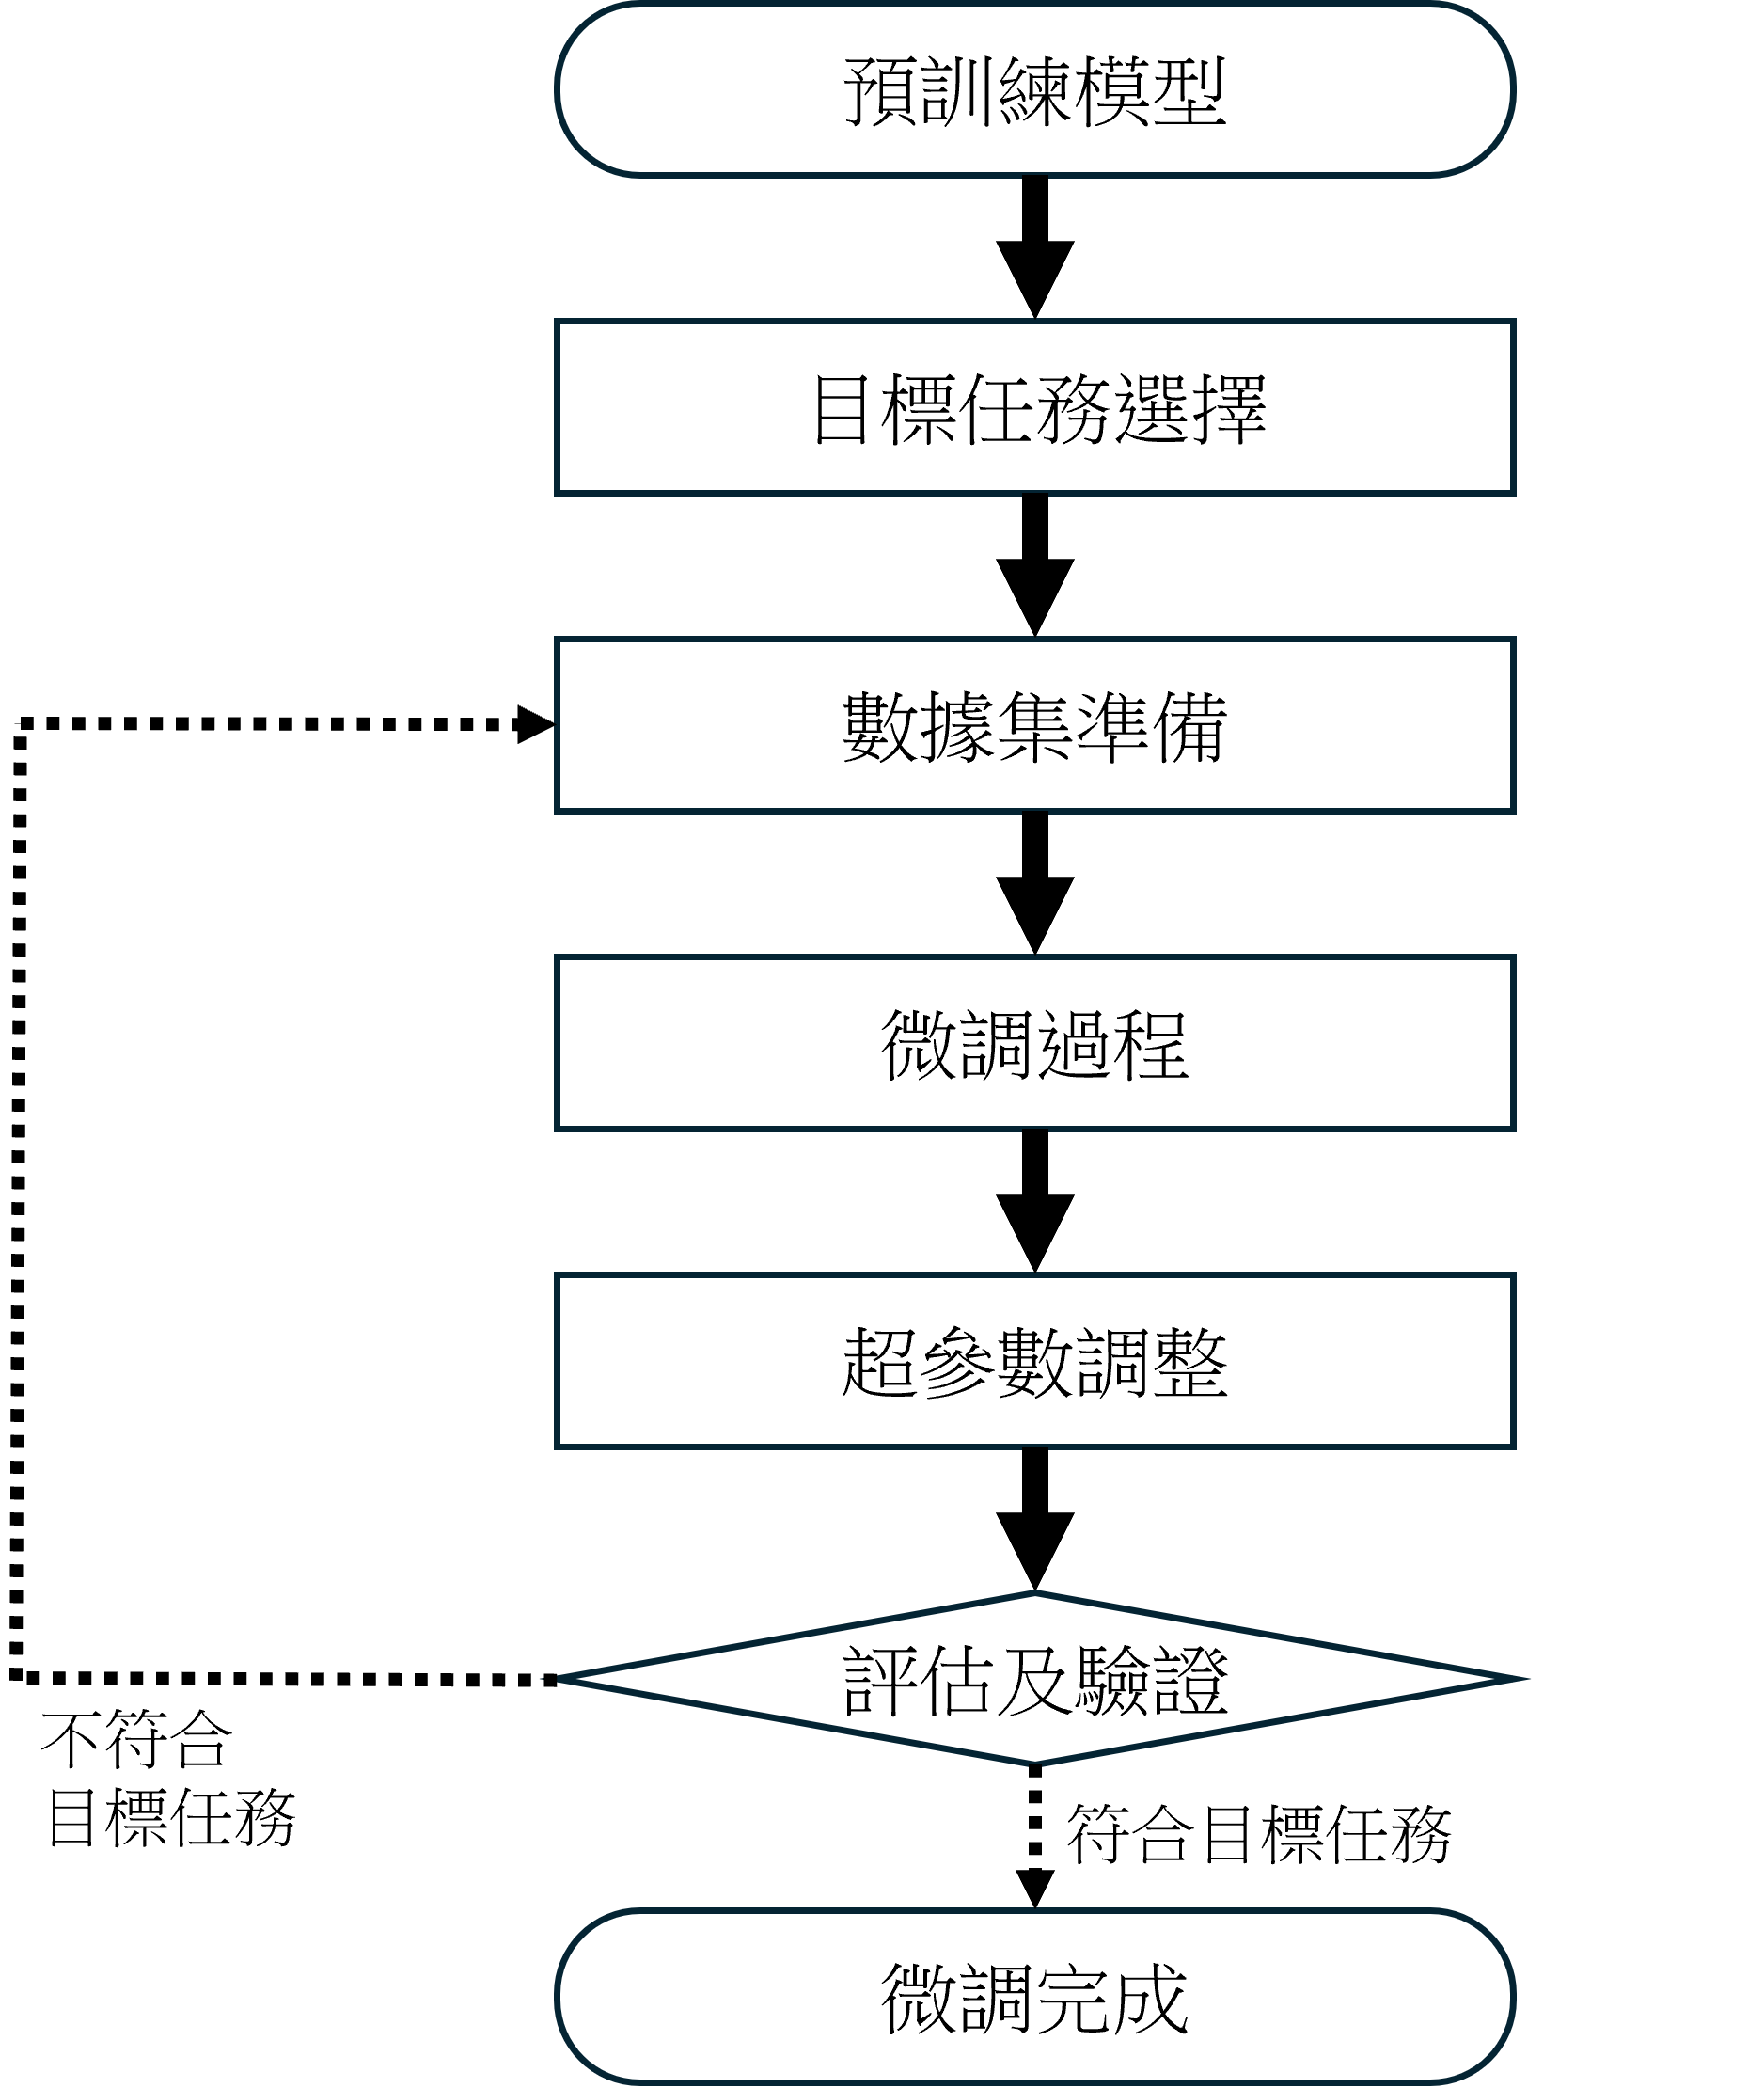
\includegraphics[scale=0.9]{flowcahrt}
		\caption{研究流程設計概念圖}
	\end{figure}
	
	\CJKfakebold{\textbf{預訓練模型}}:微調,顧名思義,是調整一些小部分,保留原來的大部分。由於訓練一個全新的語言模型太過耗時、耗能,要訓練一個如同ChatGPT等級的語言模型,需要上億筆資料,動輒訓練好幾個月(在耗費極大量運算資源的情況下),大多數的模型開發者都無法使用這樣的資源,也無法取得如此龐大的數據量。於是,微調他人訓練好的語言模型便成了一個選項,「站在巨人的肩膀上,使我們能夠看得更遠。」
	
	\CJKfakebold{\textbf{目標任務選擇}}:我們需要有一個明確的目標,我們要把模型微調成什麼樣子。要擁有更強的語言表達能力?還是要增加一些他本來沒有的東西?要先把目標確立,才可以進行之後的動作。
	
	\CJKfakebold{\textbf{數據集準備}}:準備大量的數據(使用者與目標模型的對話),每一組數據,都要是我們希望目標模型在使用者輸入語句後的回應。這些數據之於目標模型就像陽光之於植物,都是成長不可或缺的養分。
	
	\CJKfakebold{\textbf{微調過程}}:微調的過程最重要的東西,叫做「權重」,權重代表了語言模型對某件事情的重要性,權重越高,重要性也就越高。
	用國文段考來舉例好了,課本裡面有15篇論語的小篇章,老師說其中4篇會考默書,其他11篇根本不會在考題上出現,那4篇學生是不是就會拚命看、拚命背?其他的11篇是不是相對地,只是稍微看一下,甚至根本沒去看?此時,在學生心目中,需要考默書的那4篇的權重相對於其他11篇,就高上了許多。
	微調的過程,會有三個權重:初始權重、變化權重、以及最終權重。初始權重,是預訓練模型的權重;變化權重,是以我們準備的數據集微調模型後的權重;而最終權重,則是把上述兩種權重加起來得出的結果,也是我們最終微調完的模型。
	
	\CJKfakebold{\textbf{超參數調整}}:我們可以透過調整一些參數,來使結果更加理想。我們通常會調整的超參數有:訓練次數(Number of Epochs)、正規化參數(Regularization)、批次大小(Batch Size)等:
	\begin{wrapfigure}{r}{.4\textwidth}
		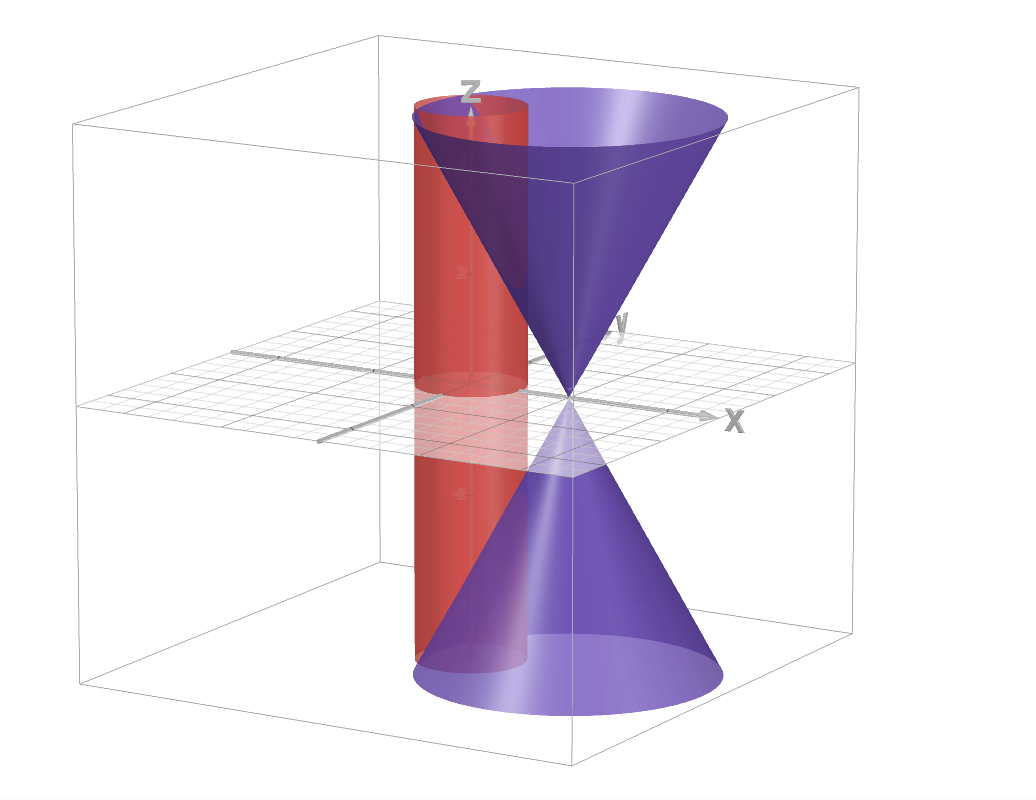
\includegraphics[width=.4\textwidth]{penalty}
		\caption{正規化參數調整示意圖}
		\label{fig:reg}
	\end{wrapfigure}
	\begin{itemize}
		\item 訓練次數過少可能會造成訓練不足,
		就跟考試裸考沒什麼兩樣;
		過多則會使回答太過趨近於訓練資料而缺乏變通性。
		\item 正規化參數(又稱為正則化參數),透過懲罰機制阻止模型過度趨近於訓練資料(即過擬合,overfitting),常見的兩種方法為L1正規化以及L2正規化,兩者的計算方式為$L1 Penalty:\lambda\sum_{i=1}^{d}|w_i|;L2 Penalty:\lambda\sum_{i=1}^{d}w^2_i$,正規化的圖形化如圖\ref{fig:reg}:透過圓錐和圓柱的交集增加損失,避免過擬合。
		

	
		\item 批次大小,將數據集分成好多塊後每一塊的資料量;批次大小越大,換句話說,資料被切越少刀,我們訓練出來的結果就越穩定,相對地,耗時也較久,效率不佳;在效率與穩定之間求取平衡,是我們須重視的點。
	\end{itemize}
	
	\CJKfakebold{\textbf{評估及驗證}}:微調完畢後的模型要經過標準化評估,以確認微調是否成功。常見方法如本次研究中使用的問題集比對、意識測驗。
	
	本研究注重在微調部份,故超參數為本次實驗的固定變因,整理後本實驗大致可分為三個階段:\textbf{資料前處理}、\textbf{微調模型訓練}、\textbf{測驗},整體流程如下:
	
	\begin{figure}[H]
		\centering
	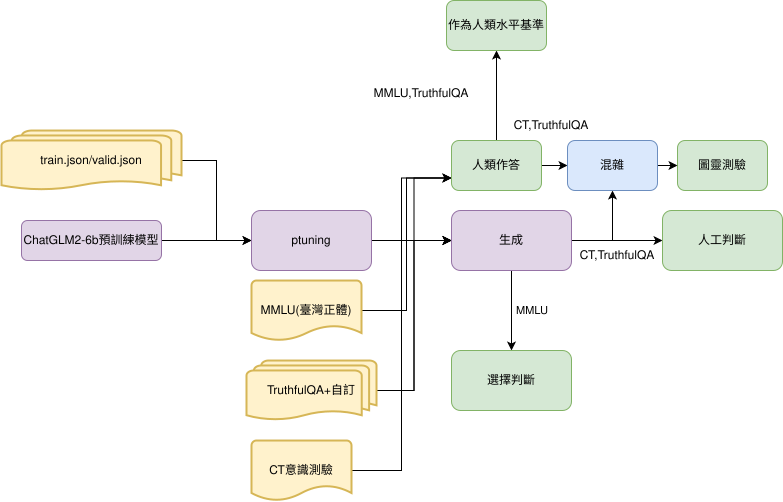
\includegraphics[width=\textwidth]{flowofstudy}
	\caption{研究流程圖}
	\end{figure}
	
	\subsubsection{(二)、資料前處理}
	此部份包含測試資料的取得、題目的翻譯和校正、決定題目的評鑑指標。此部份均由人工處理,本次的資料來源是由研究人員從網路上抓取可信資料並加上情緒特徵,表現出特定角色特色,所有需要處理的資料處理流程如下:
	\begin{figure}[H]
		\centering
		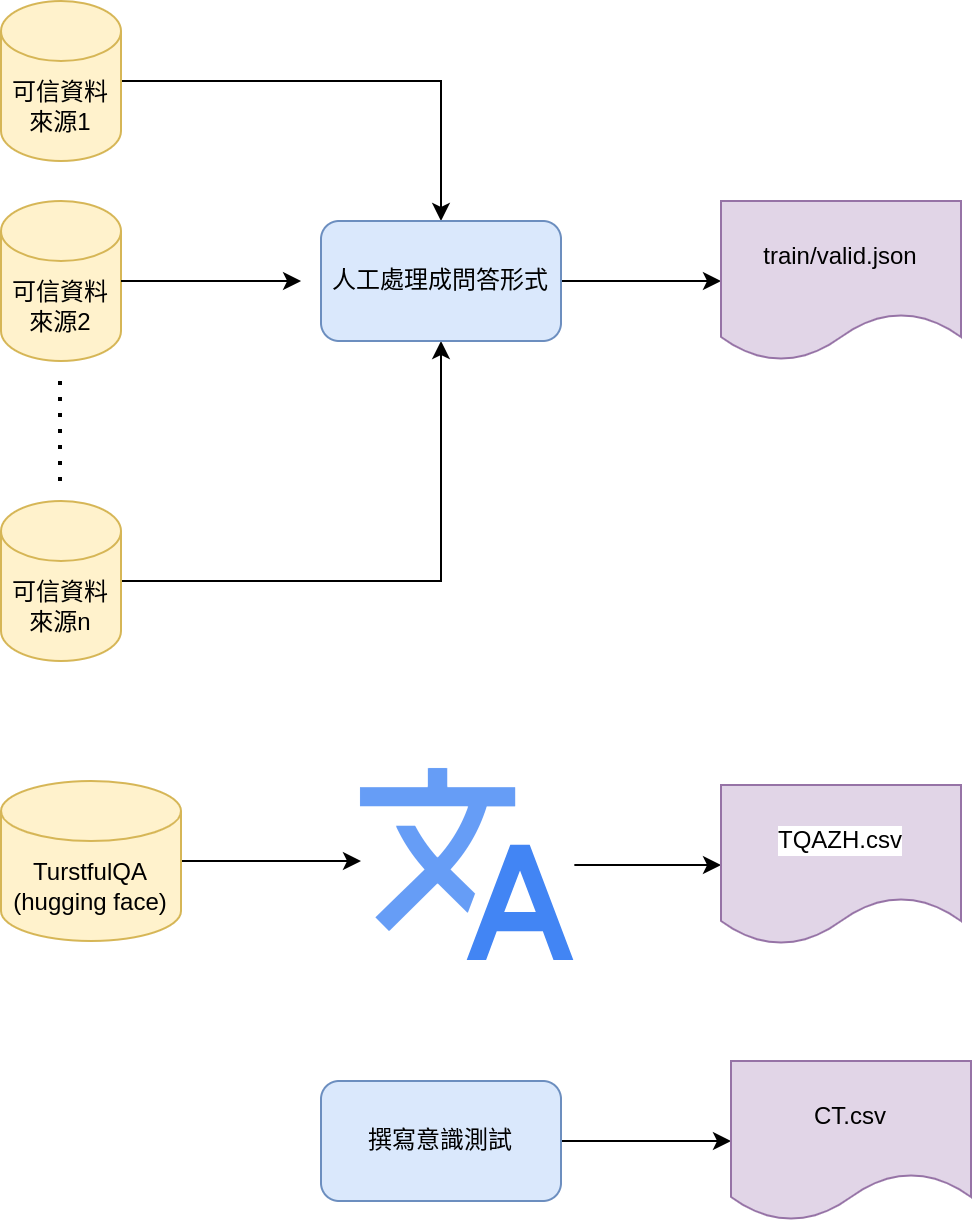
\includegraphics[scale=0.3]{dataprocess}
		\caption{資料前處理流程圖}
	\end{figure}
	\subsubsection{(三)、微調模型訓練}
	資料均正規化之後被模型用以微調,本次實驗採用的最多總共有3000步(max\_steps=3000) ,每500次紀錄一次,為保持固定變因,每次微調時參數設定均相同
%	,相關參數紀錄如下:
%	\begin{itemize}
%		\item gradient\_accumulation\_steps: 16
%		\item learning\_rate: 0.01
%		\item pre\_seq\_len: 128
%	\end{itemize}
	\subsubsection{(四)、測驗}
	訓練完成後,模型會依照指示生成出評估內容,結果評估會使用前一小節討論的兩種指標(TrustfulQA、意識測試)評估,各指標依據測驗目的不同將會分別陳列。
	\subsection{三、變項探討與實驗設計}
	本研究可以分為以下4個實驗:
	\subsubsection{(一)、訓練次數對資料正確性的影響}
	\CJKfakebold{\textbf{操作}}:紀錄不同訓練次數(steps)的模型在TrustfulQA中的表現。
	
	\CJKfakebold{\textbf{紀錄}}:BLEU、ROUGE1、ROUGE2、ROUGEL分數。
	
	\CJKfakebold{\textbf{分析}}:由不同訓練次數找出其輸出對於一般知識的正確性。
	
	\subsubsection{(二)、模型版本對資料正確性的影響}
	\CJKfakebold{\textbf{操作}}:紀錄不同版本的模型在TrustfulQA中的表現。

	\CJKfakebold{\textbf{紀錄}}:BLEU、ROUGE1、ROUGE2、ROUGEL分數。

	\CJKfakebold{\textbf{分析}}:由不同模型版本找出其輸出對於一般知識的正確性。
	
	\subsubsection{(三)、訓練次數對角色意識的影響}
	\CJKfakebold{\textbf{操作}}:紀錄不同訓練次數的模型在意識測試(CT)中的表現並依據標準意識測試評分表人工計算分數。

	\CJKfakebold{\textbf{紀錄}}:依據標準意識測試評分表中得出的絕對分數。

	\CJKfakebold{\textbf{分析}}:由不同訓練次數找出其輸出表現角色意識的程度。
	
	\subsubsection{(四)、模型版本對角色意識的影響}
	\CJKfakebold{\textbf{操作}}:紀錄不同版本的模型在意識測試(CT)中的表現並依據標準意識測試評分表人工計算分數。

	\CJKfakebold{\textbf{紀錄}}:依據標準意識測試評分表中得出的絕對分數。

	\CJKfakebold{\textbf{分析}}:由不同模型版本找出其輸出表現角色意識的程度。
	\section{肆、研究結果}
	經過微調後(實際訓練過程如下圖所示\footnote{為確保公平性,此圖中有關使用者資料被抹除}):
	
	\begin{figure}[H]
		\centering
		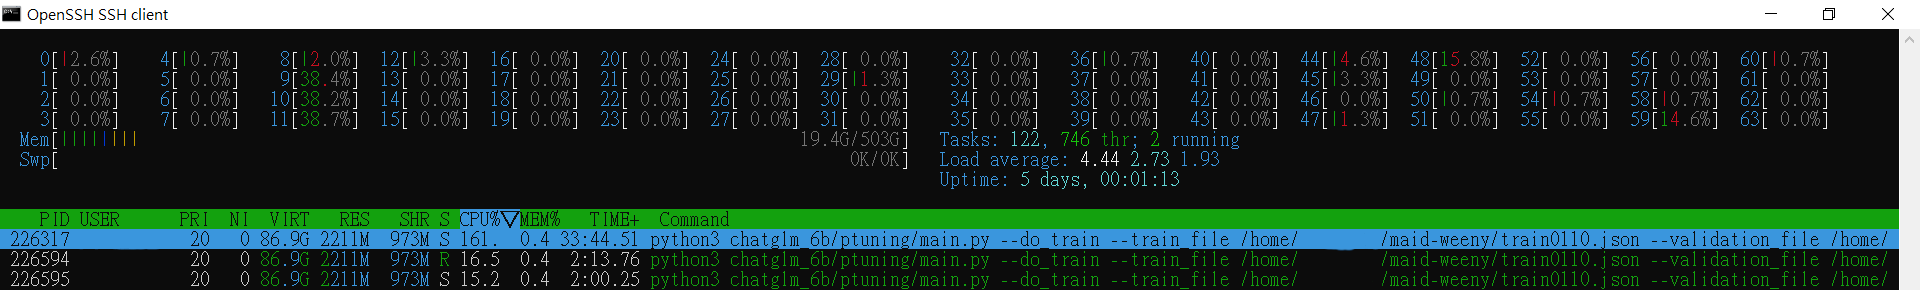
\includegraphics[width=\textwidth]{running}
		\caption{實際微調狀況}
	\end{figure}

	經過第參章第一節第五小節描述的測驗方法評估,為保持圖表簡潔,繪圖時以1-1代替ChatGLM1、檢查點500;1-2代替ChatGLM1、檢查點1000;測驗結果分類陳列如下:%maybe change max token:)

%	
	%人工討論6*100?
	%標準比對
%	\subsection{一、自我測試比較}
%	此處的結果為模型輸出和範例測試資料比較的結果,但需要注意的是,部份範例測試資料旨在評估開放性問答,即可能有多種回答方式的問題,故不應該以此判斷模型成效。
%	\begin{table}[H]
%		\centering
%		\caption{ChatGLM1模型自我測試結果}
%		\begin{tabular}{lllll}
%			     & BLEU-4 & ROUGE-1 & ROUGE-2 & ROUGE-L \\
%			500  & 3.5707 & 18.972  & 4.1165  & 14.8251 \\
%			1000 & 2.0272 & 18.727  & 3.351   & 11.7919 \\
%			1500 & 9.2931 & 25.5811 & 11.3775 & 23.4718 \\
%			2000 & 3.2251 & 18.8774 & 2.966   & 14.5734 \\
%			2500 & 5.9346 & 23.1986 & 5.332   & 19.5588 \\
%			3000 & 4.2043 & 19.2612 & 3.755   & 16.4394
%		\end{tabular}
%	\end{table}

	\subsection{一、TruthfulQA(開放式問答)}
	
	
	\parbox{\textwidth}{
	\subsubsection{(一)、比較第一版模型不同訓練次數}


	
	
	\CJKfakebold{結果}:第一版模型中不同訓練次數對資料正確性的影響如下表所示:
	
	
	\begin{table}[H]
		\centering
		\begin{tabular}{>{\hspace{0pt}}m{0.162\textwidth}>{\hspace{0pt}}m{0.181\textwidth}>{\hspace{0pt}}m{0.185\textwidth}>{\hspace{0pt}}m{0.185\textwidth}>{\hspace{0pt}}m{0.185\textwidth}} 
			\toprule
			檢查點 & BLEU-4 & Rouge1 & Rouge2 & RougeL  \\ 
			\hline
			原始   & 0.033  & 0.033  & 0.014  & 0.033   \\
		500   & 0.038  & 0.031  & 0.013  & 0.031   \\
		1000   & 0.038  & 0.034  & 0.012  & 0.034   \\
		1400   & 0.035  & 0.035  & 0.011  & 0.035   \\
		2000  & 0.036  & 0.033  & 0.009  & 0.033   \\
		2500  & 0.037  & 0.031  & 0.010   & 0.031   \\
		3000  & 0.035  & 0.032  & 0.011  & 0.032   \\
			\bottomrule
		\end{tabular}
	\caption{第一版模型中不同訓練次數對資料正確性的影響}
	\end{table}
	
		\begin{wrapfigure}{r}{0.6\textwidth}
		\centering
		
\includegraphics[width=0.6\textwidth]{1vc}
		\caption{第一版模型中不同訓練次數對資料正確性的影響}
	\end{wrapfigure}

	\CJKfakebold{發現}:
	
	

	\begin{enumerate}
		\item ChatGLM1知識的整體表現不會因為微調而有明顯改變
		\item Rouge1和RougeL分數極為相近
		\item 採用BLEU-4作為評分分數會顯高於原始模型
	\end{enumerate}


	\CJKfakebold{思考}:BLEU-4分數之所以高於原始模型可能是因為生成長度較原本模型長,進而使得其BP分數達到極限(即$BP=1$)。

}

\parbox{\textwidth}{

	\subsubsection{(二)、比較第二版模型不同訓練次數}

	
	\CJKfakebold{結果}:第二版模型中不同訓練次數對資料正確性的影響如下表所示:
	


\begin{table}[H]
	\centering
	\begin{tabular}{>{\hspace{0pt}}m{0.137\textwidth}>{\hspace{0pt}}m{0.187\textwidth}>{\hspace{0pt}}m{0.19\textwidth}>{\hspace{0pt}}m{0.19\textwidth}>{\hspace{0pt}}m{0.19\textwidth}} 
		\toprule
		檢查點 & BLEU-4 & Rouge1 & Rouge2 & RougeL  \\ 
		\hline
		原始    & 0.038  & 0.035  & 0.014  & 0.035   \\
		500    & 0.041  & 0.031  & 0.011  & 0.031   \\
		1000    & 0.026  & 0.011  & 0.004  & 0.011   \\
		1500    & 0.054  & 0.024  & 0.006  & 0.024   \\
		2000    & 0.046  & 0.030   & 0.009  & 0.03    \\
		2500    & 0.021  & 0.009  & 0.003  & 0.009   \\
		3000    & 0.031  & 0.022  & 0.009  & 0.022   \\
		\bottomrule
	\end{tabular}
\caption{第二版模型中不同訓練次數對資料正確性的影響}
\end{table}

\begin{wrapfigure}{r}{0.6\textwidth}
	\centering
	
\includegraphics[width=0.6\textwidth]{2vc}
	\caption{第二版模型中不同訓練次數對資料正確性的影響}
\end{wrapfigure}


	\CJKfakebold{發現}:

	\begin{enumerate}
		\item ChatGLM2知識的整體表現因微調而有略為減低
		\item 1000及2500檢查點的表現特別低落
		\item Rouge表現均不如原始模型
	\end{enumerate}



	\CJKfakebold{思考}:模型本身經過微調,其原本知識可能有些微下降,但就目前數據而言影響並不大。這是已知現象,此現象又稱為概念遺忘,且目前許多微調方法都會產生這種嚴重的副作用。\cite{mukhoti2023finetuning}

}

\parbox{\textwidth}{
	
	\subsubsection{(三)、比較第三版模型不同訓練次數}
	

	
	\CJKfakebold{結果}:第三版模型中不同訓練次數對資料正確性的影響如下表所示:
	
	
	\begin{table}[H]
		\centering
		\begin{tabular}{>{\hspace{0pt}}m{0.159\textwidth}>{\hspace{0pt}}m{0.179\textwidth}>{\hspace{0pt}}m{0.182\textwidth}>{\hspace{0pt}}m{0.182\textwidth}>{\hspace{0pt}}m{0.182\textwidth}} 
			\toprule
			檢查點 & BLEU-4 & Rouge1 & Rouge2 & RougeL  \\ 
			\hline
			原始   & 0.036  & 0.037  & 0.012  & 0.036   \\
			500   & 0.037  & 0.012  & 0.002  & 0.012   \\
			1000   & 0.038  & 0.011  & 0.000    & 0.011   \\
			1500   & 0.021  & 0.004  & 0.000    & 0.004   \\
			2000   & 0.019  & 0.006  & 0.000    & 0.006   \\
			2500   & 0.014  & 0.003  & 0.000    & 0.003   \\
			3000   & 0.014  & 0.003  & 0.000    & 0.003   \\
			\bottomrule
		\end{tabular}
	\caption{第三版模型中不同訓練次數對資料正確性的影響}
	\end{table}
	
	\begin{wrapfigure}{r}{0.6\textwidth}
		\centering
		
\includegraphics[width=0.6\textwidth]{3vc}
		\caption{第三版模型中不同訓練次數對資料正確性的影響}
	\end{wrapfigure}
	
	\CJKfakebold{發現}:
	
	

	\begin{enumerate}
		\item ChatGLM3知識的整體表現因微調而有顯著降低的現象
		\item 1000檢查點之後知識表現明顯下降
		\item Rouge1、Rouge2及RougeL分數均顯低於原始模型
		\item Rouge2的分數部份為0
	\end{enumerate}



	\CJKfakebold{思考}:模型本身經過微調,其原本知識有明顯下降,驗證了上一個實驗發現的現象。另外Rouge2分數為零可能是因為此版本的回覆幾乎沒有回答到問題,尤其是檢查點1500以後全部都是微調的資料,失去原本的內容,其他分數較低的現象亦是因為此原因。

}

\parbox{\textwidth}{

	\subsubsection{(四)、比較相同訓練次數的三版模型}
	
	\CJKfakebold{結果}:三版模型中相同訓練次數對資料正確性的影響如下圖所示:
	
		\begin{figure}[H]
		\centering
		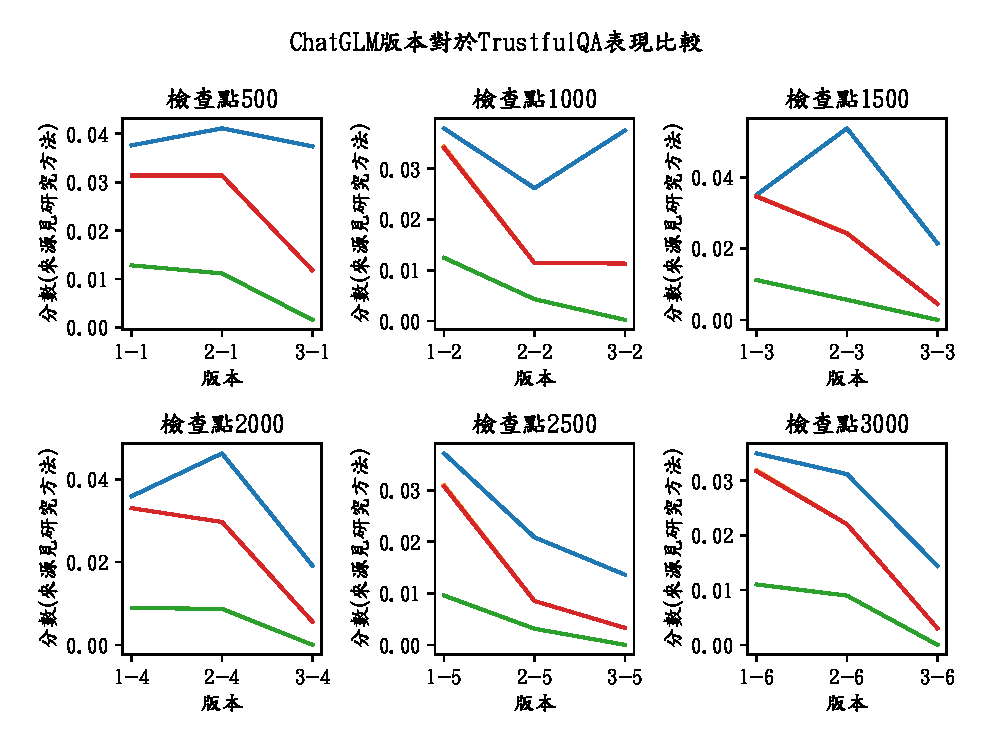
\includegraphics[width=0.8\textwidth]{allcomp}
		\caption{三版模型中相同訓練次數對資料正確性的影響}
	\end{figure}
	
	\CJKfakebold{發現}:
	
	

	\begin{enumerate}
		\item 檢查點1000以上的模型表現結果會因模型版本而有不同程度的降低
		\item 整體而言第三版的表現均較其他兩版差
	\end{enumerate}



	\CJKfakebold{思考}:三版模型訓練後表現均有所下降,惟第三版下降較多,這可能是因為第三版的資料量較大,較容易被微調的資料混淆,導致原本的知識表現下降。訓練時宜以更多更細節的資料微調,使其不會因為資料故於廣泛而混淆。
	
}

%	\subsection{三、MMLU(封閉性單一選擇問答)}
	\subsection{二、CT 自我意識測驗}
	
	\parbox{\textwidth}{
		
	\subsubsection{(一)、比較第一版模型不同訓練次數}
	\CJKfakebold{結果}:第一版模型中不同訓練次數對意識表現的影響如下表所示:
	
	
	\begin{table}[H]
		\centering
		\begin{tabular}{>{\hspace{0pt}}m{0.107\textwidth}|>{\hspace{0pt}}m{0.107\textwidth}|>{\hspace{0pt}}m{0.107\textwidth}|>{\hspace{0pt}}m{0.134\textwidth}|>{\hspace{0pt}}m{0.134\textwidth}|>{\hspace{0pt}}m{0.134\textwidth}|>{\hspace{0pt}}m{0.134\textwidth}}
			原始 & 500 & 1000 & 1500  & 2000  & 2500  & 3000   \\ 
			\hline
			6.0 & 6.0 & 9.0 & 10.0 & 12.0 & 14.0 & 13.0 
		\end{tabular}
		\caption{第一版模型中不同訓練次數對意識表現的影響}
	\end{table}
	
	\begin{wrapfigure}{r}{0.6\textwidth}
		\centering
		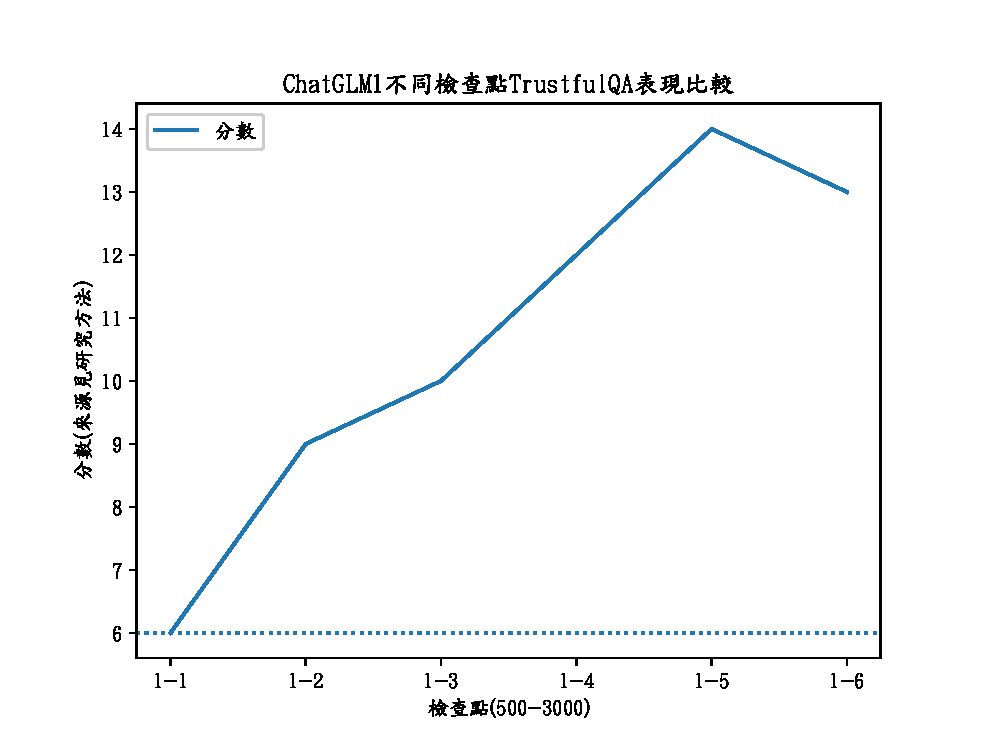
\includegraphics[width=0.6\textwidth]{1ctc}
		\caption{第一版模型中不同訓練次數對意識表現的影響}
	\end{wrapfigure}
	
	\CJKfakebold{發現}:
	
	
	

	\begin{enumerate}
		\item 經過微調可以有效提高意識表現的分數
		\item 其中以2500次為最佳,之後可能會產生衰減的現象
		\item 隨著訓練次數增加,其成果表現也較佳
	\end{enumerate}



	\CJKfakebold{思考}:本次微調能夠有效增進其意識表現,且隨著次數增加,分數有明顯成長。
	
	}

\parbox{\textwidth}{
	
	\subsubsection{(二)、比較第二版模型不同訓練次數}
	\CJKfakebold{結果}:第二版模型中不同訓練次數對意識表現的影響如下表所示:
	
\begin{table}[H]
	\centering
	\begin{tabular}{>{\hspace{0pt}}m{0.146\textwidth}|>{\hspace{0pt}}m{0.117\textwidth}|>{\hspace{0pt}}m{0.117\textwidth}|>{\hspace{0pt}}m{0.117\textwidth}|>{\hspace{0pt}}m{0.117\textwidth}|>{\hspace{0pt}}m{0.117\textwidth}|>{\hspace{0pt}}m{0.117\textwidth}}
		原始  & 500 & 1000 & 1500 & 2000 & 2500 & 3000  \\ 
		\hline
		13.0 & 5.0 & 8.0 & 3.0 & 3.0 & 3.0 & 9.0 
	\end{tabular}
\caption{第二版模型中不同訓練次數對意識表現的影響}
\end{table}
	
	\begin{wrapfigure}{r}{0.6\textwidth}
		\centering
		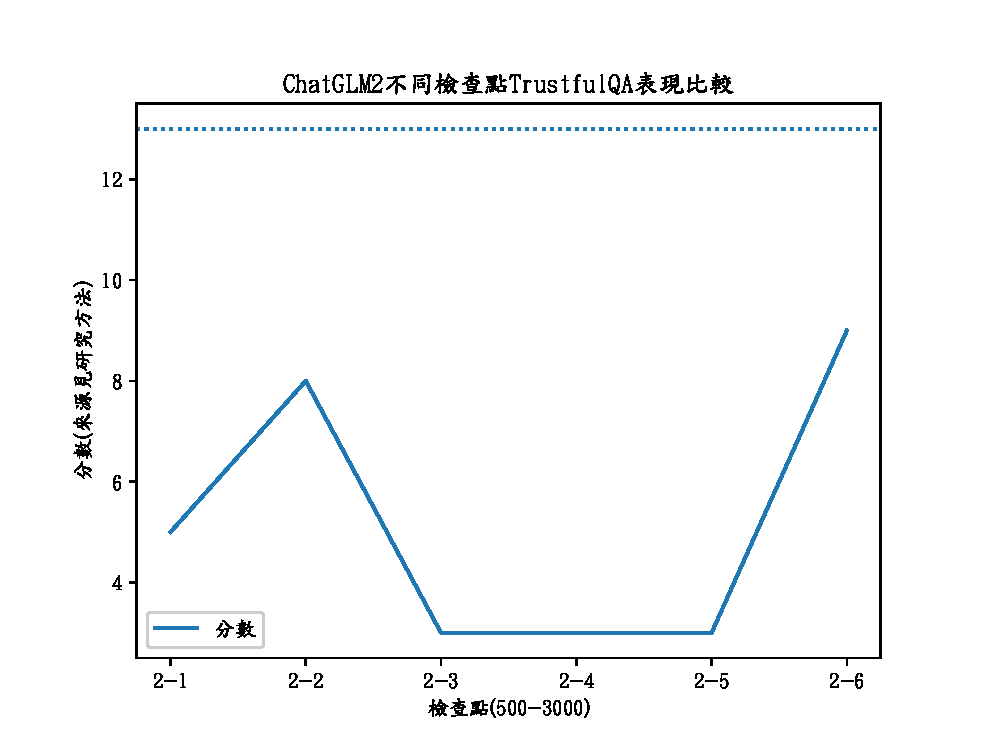
\includegraphics[width=0.6\textwidth]{2ctc}
		\caption{第二版模型中不同訓練次數對意識表現的影響}
	\end{wrapfigure}
	
	\CJKfakebold{發現}:
	
	

	\begin{enumerate}
		\item 1500、2000、2500檢查點的表現結果均不如預期
		\item 表現均不如原始模型
		\item 檢查點3000符合預期的有上升一些
	\end{enumerate}


	\CJKfakebold{思考}:有可能第二版的原始模型資料量較大,而微調資料量太少而導致表現不佳。
	
	}

\parbox{\textwidth}{
	
	\subsubsection{(三)、比較第三版模型不同訓練次數}
	\CJKfakebold{結果}:第三版模型中不同訓練次數對意識表現的影響如下表所示:
	
	\begin{table}[H]
		\centering
		\begin{tabular}{>{\hspace{0pt}}m{0.138\linewidth}|>{\hspace{0pt}}m{0.111\linewidth}|>{\hspace{0pt}}m{0.111\linewidth}|>{\hspace{0pt}}m{0.111\linewidth}|>{\hspace{0pt}}m{0.111\linewidth}|>{\hspace{0pt}}m{0.138\linewidth}|>{\hspace{0pt}}m{0.138\linewidth}}
			原始  & 500 & 1000 & 1500 & 2000 & 2500  & 3000   \\ 
			\hline
			14.0 & 8.0 & 9.0 & 9.0 & 4.0 & 11.0 & 15.0 
		\end{tabular}
	\caption{第三版模型中不同訓練次數對意識表現的影響}
	\end{table}
	
	\begin{wrapfigure}{r}{0.6\textwidth}
		\centering
		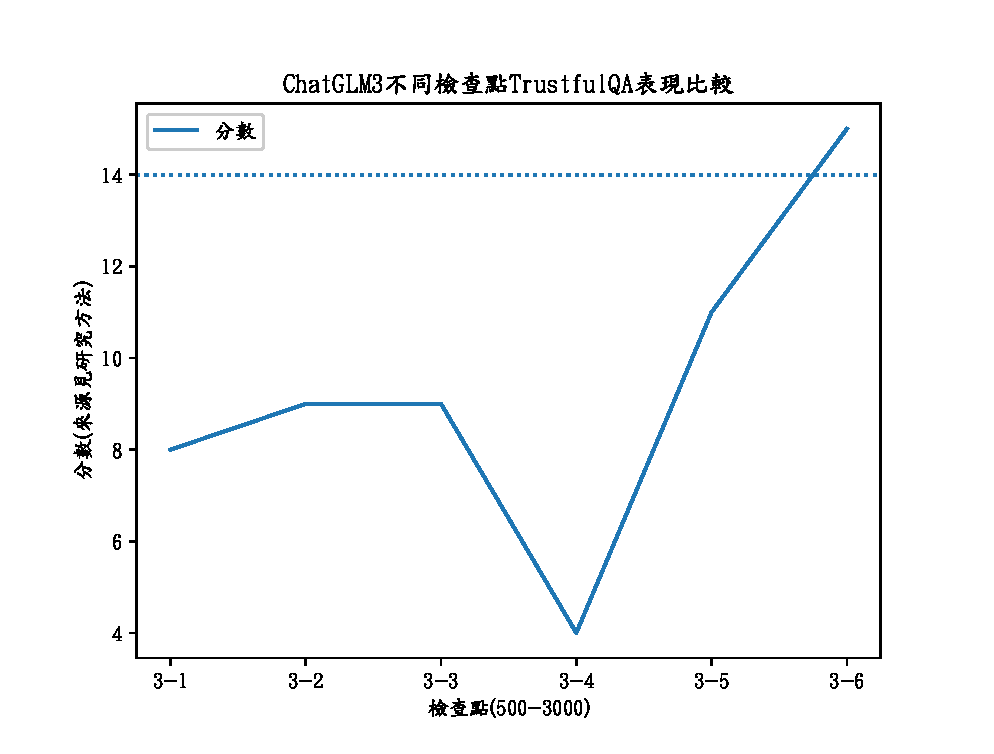
\includegraphics[width=0.6\textwidth]{3ctc}
		\caption{第三版模型中不同訓練次數對意識表現的影響}
	\end{wrapfigure}
	
	\CJKfakebold{發現}:
	
	

	\begin{enumerate}
		\item ChatGLM3多數情感表現不如原始模型
		\item 檢查點3000超越原始模型
		\item 整體大致呈現隨訓練次數上升而有較好的表現
	\end{enumerate}



	\CJKfakebold{思考}:模型確實有因為微調而表現出更多的角色意識和情感,且大致隨訓練次數增加而增加。
	
	}

\parbox{\textwidth}{
	
	\subsubsection{(四)、比較相同訓練次數的三版模型}
	\CJKfakebold{結果}:三版模型中相同訓練次數對意識表現的影響如下圖所示:
	
	\begin{figure}[H]
		\centering
		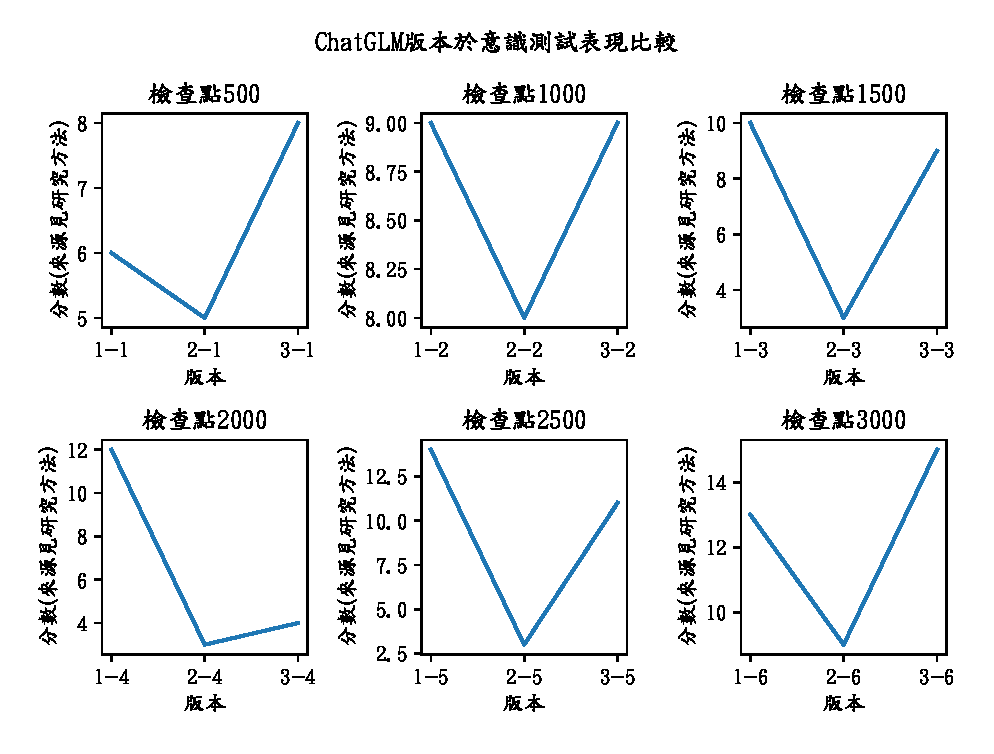
\includegraphics[width=.7\textwidth]{alltccomp}
		\caption{三版模型中相同訓練次數對意識表現的影響}
	\end{figure}
	
	\CJKfakebold{發現}:
	
	

	\begin{enumerate}
		\item 檢查點1000以上的模型表現結果會因模型版本而整體來說降低
		\item 整體而言第二版的表現均較其他兩版差
		\item 第三版表現顯著的優異
	\end{enumerate}



	\CJKfakebold{思考}:此次表現以第三版表現最佳,其中第二版的輸出經檢視後有不少不具實際意義的回覆,如空白、單字、不完整句意等情況。
	
%	\subsection{五、圖靈測驗}
%	此模型在圖靈測驗中表現經整理成混淆矩陣後\footnote{轉換為百分比表示}(下表),其準確率可以高達、F1 score可以高達。
}

	\section{伍、討論}
	
	綜合上述實驗,將結果整合繪製成以下兩張圖表:
	
	\begin{figure}[H]
		\centering
		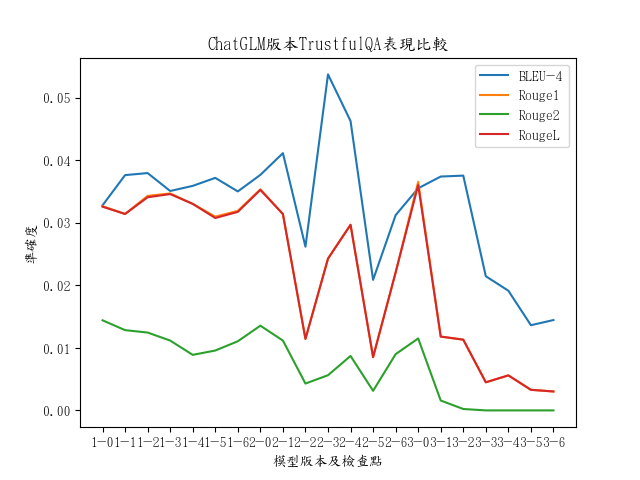
\includegraphics[width=.5\textwidth]{mixscorenew}
		\caption{綜合不同模型及檢查點在TrustfulQA中的表現}
		\label{pic1:mixtscore}
	\end{figure}

	\begin{figure}[H]
		\centering
		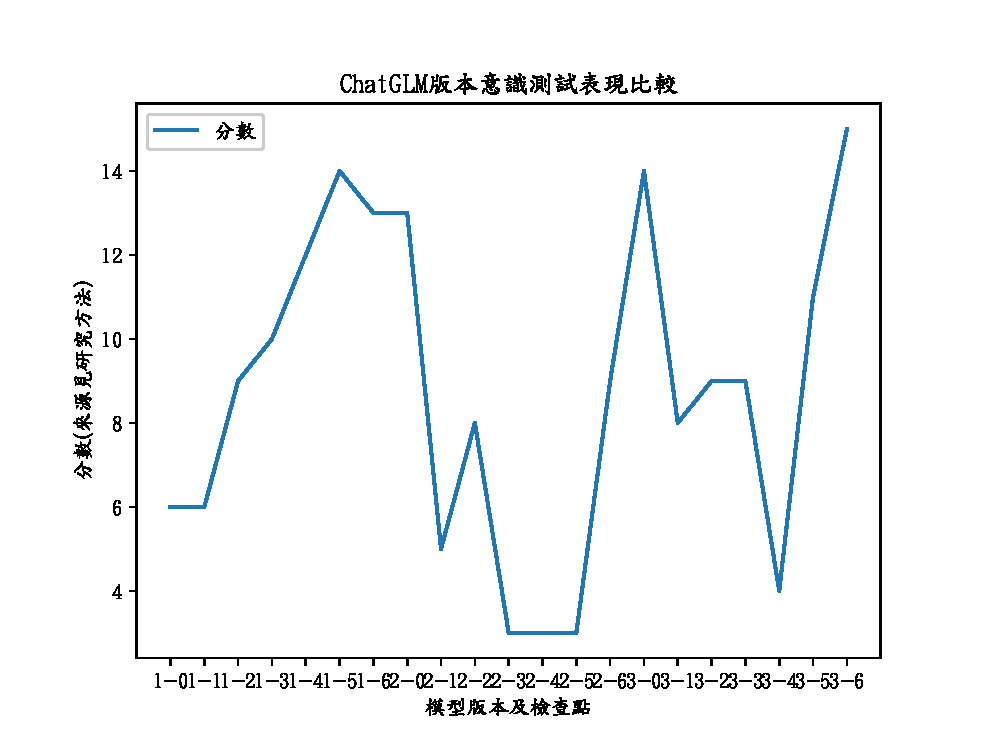
\includegraphics[width=.5\textwidth]{mixctscore}
		\caption{綜合不同模型及檢查點在意識測試中的表現}
		\label{pic2:mixcscore}
	\end{figure}

	\subsection{一、不同檢查點比對}
	
	\subsubsection{(一)、事實正確性}
	探討圖\ref{pic1:mixtscore}中的現象:
	
	\begin{itemize}
		\item 第二版的第1000和2500檢查點存在顯著波動。
		\item 微調過多次會導致他的表現下降,符合<Fine-tuning can cripple your foundation model; preserving features may be the solution>\cite{mukhoti2023finetuning}的研究,和理論相符,均會在多次訓練後原有知識表現下降。
%		\item 回答有關我們給予的微調資料時能夠提供正確的回覆。
		\item 第一版模型訓練後表現較第三版模型好,可能是因為我們我們本次實驗所提供的資料集相對於模型原有的資料過少,而對原本模型造成混淆的現象,但因第一版的資料量較少所以較不容易造成混淆,而第三版中因為模型原有資料量過大所以導致我們混淆了原本的模型而使其表現較差。
	\end{itemize}

	\subsubsection{(二)、意識測試}
	探討圖\ref{pic2:mixcscore}中的現象:
	
	\begin{itemize}
		\item 不同版本之間存在巨大的波動。
		\item 整體而言意識表現均隨者訓練次數增加而增壓。
		\item 第二版模型表現較差,但3000檢查點的性能仍和其他版本該檢查點的形能相近。
	\end{itemize}
	
	
	\subsection{二、不同模型比對}
	探討不同模型之間兩測驗性能比較:
	
	\begin{itemize}
		\item 微調後的ChatGLM2的在事實正確性及意識測試中表現為三者之中最差。
		\item 整體而言模型隨訓練次數增加,在兩個測驗中分數皆隨之增加,符合理論預測。
		\item ChatGLM3微調後部份表現不如ChatGLM,此現象係因ChatGLM3訓練前資料量比ChatGLM多,而微調增加的資料量在第一版中較為顯著,所以較不會造成混淆的情況。
		\item 事實正確性分數較高的模型其情感表現較差(第二版),反之亦同(第三版)。
	\end{itemize}
	
%	\subsection{二、和人類表現比對}
%check two relation between knwoledge and ct do a simple linaer regression
	\subsection{三、未來展望}
	%	\begin{quote}
	%		We can only see a short distance ahead, but we can see plenty there that needs to be done.	\newline--
	%	\end{quote}
	\epigraph{	We can only see a short distance ahead, but we can see plenty there that needs to be done.}{\textit{艾倫圖靈}}
%	本次研究時間較為緊湊,未能完成更多類型模型及微調器的比較和對照實驗,實屬可惜,且若可取得更多有關數據集可以更準確的評估訓練效果。本研究往後將進一步以採用其他模型及更多數據資料集進行研究。

	本實驗雖已做出相當可觀的研究成果,但受限於資源及時間,離目標還有一段距離,從趨勢看來,修正自然語言模型審查機制確實可行,本研究往後將進一步朝以下目標繼續研究:
	
	\begin{itemize}
		\item 更完整的訓練資料集,蒐羅更多有關的可信資料集作為基礎。
		\item 更全面、標準的評估方式,取得更多有關數據集以更準確的評估訓練效果。
		\item 加入超參數調整,調整訓練的正規劃參數、批次大小等。
	\end{itemize}

	\section{陸、結論}
	本次實驗我們訓練ChatGLM的三個版本,並以意識測試(CT)及TrustfulQA作為測試標準,綜合比較了不同版本語言模型微調後的結果,並分析出以下結論:
		\begin{enumerate}
			\item 我們透過訓練三個不同版本的模型,觀察到因為原始模型資料量相對於微調的資料量大小顯著性差異而導致第一版模型訓練後表現較第三版模型好
			\item 資訊正確性最高為:ChatGLM2,檢查點1500模型,其BELU分數為:0.053,資料正確性損失較小,且可對特定審查內容提供正確答覆,足顯可改善立場偏頗、缺乏資訊的問題
			\item 意識測試(CT)最高可達15分,其結果十分接近於人類真實的意識形態
		\end{enumerate}
	%https://reurl.cc/v0vaKa (L1, L2正規化)
	%	\printbibliography
	\section{柒、參考文獻資料}
	\bibliographystyle{apacite}
	\renewcommand{\refname}{}
	\bibliography{ref}
\end{document}
